\section{Discussion}\label{6_discussion}
\begin{comment}
The present study aimed at investigating whether an interactive slackline training system, which 


- results discussion (sport activity people)

- results discussion (lateral preference)

- results discussion (gender)

- observation on study during training

- interview
\end{comment}

\subsubsection{Interaction Effects}\label{6_5_interactionEffects}
No interaction effect for group x time can be shown for any measurement variable for the ISG or the HTG.
%This means that no differences between the groups can be found in any measurements.
Therefore, the hypothesis that the interactive system shows better results than a human trainer cannot be proven with a statistically significant.
Looking at Figures~\ref{fig:6_4_standImprovement}, \ref{fig:6_4_stepsImprovement}, and \ref{fig:6_4_distanceImprovement} of the improvements for the group in each measurement, no real difference can be seen between the groups.
The ISG group is at the most time slightly better in all conditions, which is not sufficient to prove a statistically significance.
A bigger difference can be shown in terms of the right leg side for the walked steps (see Figure \ref{fig:6_4_stepsRightImprovement}) and walked distance measurements (see Figure \ref{fig:6_4_distanceRightImprovement}).
It shows that the ISG is approximately 2.5 times better for the right leg.
However the standard deviation of each group is very large, so that it is also not sufficient to have a certain significance.

Since all significance values are larger than the defined alpha value of 0.05, the null hypothesis cannot be rejected.
This means that no interaction effect can be found over time from pre to post measurements comparing the groups ISG and HTG and therefore no group is better or worse than the other one.
This can be caused by multiple reasons.
%- Übung zu kurz um unterschied festzustellen

The duration of the training could have been too short to show a statistically significant difference between the groups.
All participants learned just basic techniques of slacklining but no further slackline skill has been trained.
For learning more complex exercises and techniques especially the introduction and feedback given during the execution is very important, since these are key elements of understanding how the exercise works and how to perform it correctly.
Therefore further exercises and further training over a longer time range  could lead to a more specific result.
%The only difference lied in the effect of how to provide the subject with important information and how to give her feedback about the actual performance.

%- test in zu kurzer zeitspanne um unterschied festzustellen
Second, the participants could have been too exhausted for showing a relevant effect.
Participants trained at least 45 minutes on the slackline.
After this the post measurement has been executed.
Taking the time of the training into account, the measurement results after the training could have been affected by the exhaustion of the participants. 
As a result of that no real improvement can be showing.
%because of the training could weaken the participant and therefore show not the expected results of an improvement.
%There could be a side effect that participants won't be able to show there real improvements directly after the training due to exhaustion.

%- Unterscheidung zwischen grundlegender balancefähigkeit nicht gemacht somit randomisierte ergebnisse
%alle participants anfgäner auf slackline und keine weiteren ablancetraining bla
% aber nicht nach grundlegenden balanceskill geschaut
% ist bei jedem anders, einer is besser der andere schlechter 
% im test aufgefallen, dass es gute, mittelmäßige und schlechte participants gibt, was sich in der standardabweichung wiederspiegelt
% wennn man die in gruppen einteilen würde bzw auf darauf prüfen würde wie gut die grundlegende balancefähigkeit ist, hätte man ein eingeschränkteres ergebnis, welches die std dev verringert und somit auf signifikanz kommen könnte


Lastly, there was no distinction in general balance skill of the participants.
Subjects were chosen if they had no intermediate slackline experience or no further balance skill through special sport activities.
The results show a large standard deviation for all variables in the difference of pre to post.
This is because participants improved differently after the training respectively to their pre measurement.
Differences in the general balance characteristics for the participants have been found.
Therefore, for further studies it is recommended to test on the general balancing skill and characteristic of the participants, to minimize the chance of randomized data because of not qualified participants.

% --> differ the characteristic of balance improvement to reduce randomized data
% --> no distinction in general balance skill
%Third, all participant had to make single leg stance on a common floor and on a rolled towel, which served for validating that no participants has a balance disorder.
%Another reason could be that no grouping of general balance skill has been done.
%In the study only a general distinction of no prior slackline, further balance experience, or balance disorder has been done.

%- dennoch sehr leichter trend für ISG zu verbesserung
However a trend can be observed, that the ISG improved slightly better in numerical average than the HTG.
This could be the case, because the system's gesture recognition is less tolerant about the exercise execution than a human trainer.
Whereas a trainer provides more tolerance concerning the users exercise execution, the system has a predefined gesture database to which the user has to adapt her execution.
It leads to more trial executions, because of the strict recognition of the system.

\subsubsection{Time Effects}
The time effect seen in Table \ref{tab:6_4_mainEffects} in the column \textit{Time} shows whether it differs significantly from pre to post measurement, without considering any group (see Figure~\ref{fig:6_4_timeImprovement}).
This means the time effect is observed for all participants as one entity, like no group would exist.
The results state for all measurement conditions a significant improvement, unless for stand left.
Hereby, it is proven that the used training exercises in both groups are useful and have an effect on the learning progress of the participant.

The standing left leg showed no statistically significant result ($p$ = 0.078).
It is more difficult to hold the balance on a weaker leg, because it is less familiar with handling these situations than the primary leg.
Since slacklining is a more complex balance activity, the general balance of the trainee has to be trained with her weaker leg to show an improvement of the slackline specific training.
It can be assumed that less trained legs or participants won't show an improvement as good as legs or participants that have a certain general sense of balance.
Furthermore, the physical strain could have exhausted the functionality of the leg, since post results has been measured directly after the training.

In reverse, the right leg shows significant results.
For all participants the right leg was determined as their primary leg.
The general balance skill for this leg is given through everyday physical effort and therefore it shows more stable data for balance improvements.

\begin{figure}[htb]
	\centering
	\begin{minipage}[t]{0.32\linewidth}
		\centering
		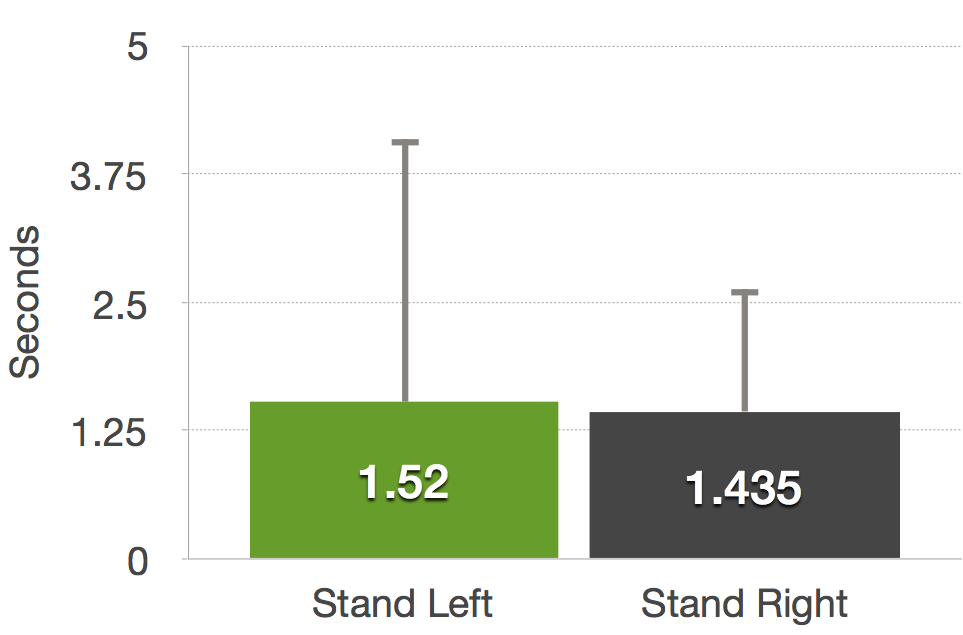
\includegraphics[width=1\linewidth]{Pictures/6_4_DIA_StandAllDiff}
		\subcaption{Time stood on the slackline}
		\label{fig:6_4_standAllDiff}
	\end{minipage}
	\hfill
	\begin{minipage}[t]{0.32\linewidth}
		\centering
		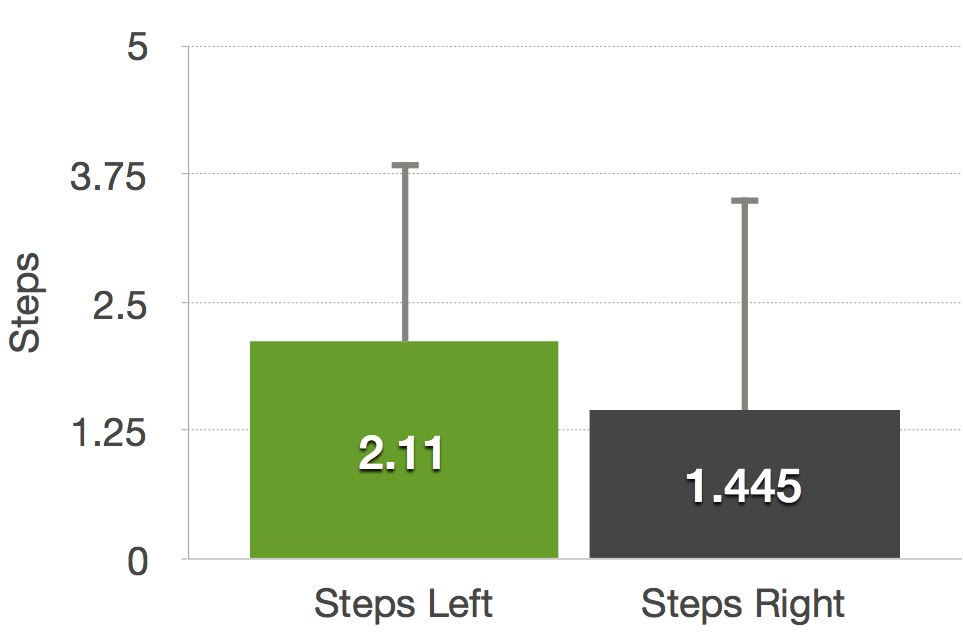
\includegraphics[width=1\linewidth]{Pictures/6_4_DIA_StepsAllDiff}
		\subcaption{Steps walked on the slackline}
		\label{fig:6_4_stepsAllDiff}
	\end{minipage}
		\hfill
	\begin{minipage}[t]{0.32\linewidth}
		\centering
		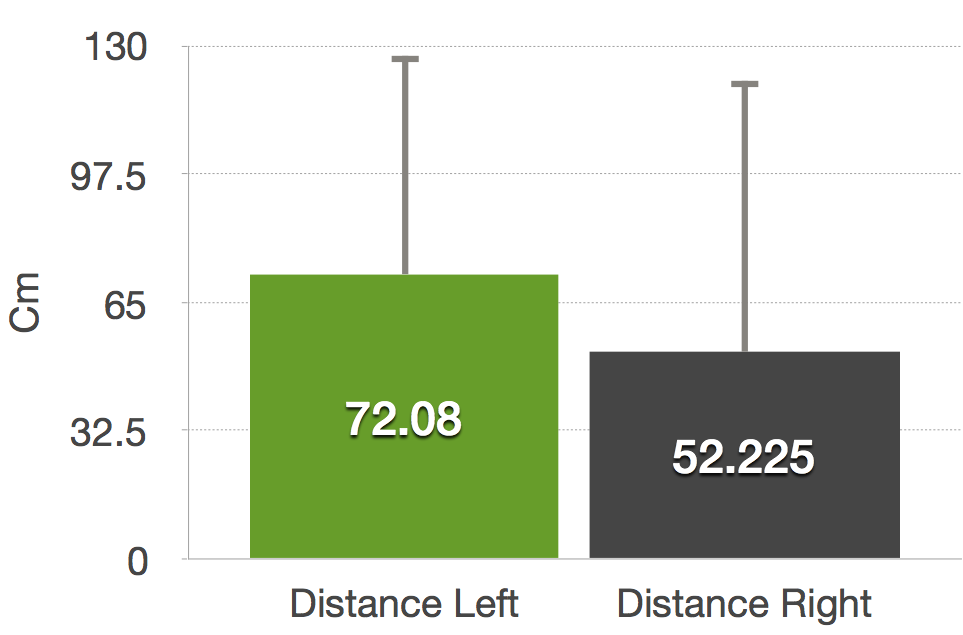
\includegraphics[width=1\linewidth]{Pictures/6_4_DIA_DistanceAllDiff}
		\subcaption{Distance walked on the slackline}
		\label{fig:6_4_distanceAllDiff}
	\end{minipage}
	\caption{Improvements of each measurement condition for the time effect}
	\label{fig:6_4_timeImprovement}
\end{figure}

\subsubsection{Group Effects}
The main effect for the group is analogue to the previous main effect of the time.
With this, the group differences can be calculated, without considering the time.
The pre and post measurements results are combined and averaged together, so the group effect over the entire time range can be obtained.
Looking at Table \ref{tab:6_4_mainEffects} in column \textit{Group}, no significant effect can be seen.
This means no group differs from each other.
The diagrams in Figure \ref{fig:6_4_mainEffectGroup} show that all results are relatively similar.
Although, the ISG is numerically slightly better than the HTG it is not sufficient to have a statistically significance difference.

The same arguments of the prior subsection \textit{\nameref{6_5_interactionEffects}} apply here as well.
Both groups were provided with the same exercise structure, description, repetitions, and time to hold the exercise.
Just the method how the information is provided to the user and the feedback during the execution of the exercise differed.
It could be the case that both training methods provide a similar amount of information and feedback such that no group was advantaged.
This again results in similar group effects.
However, it proves that both training methods show similar results and can be therefore compared with each other.
%no difference calculated
% pre nicht in betracht gezogen
%keine verbesserung der teilnehmer betrachtet
\begin{figure}[htb]
	\centering
	\begin{minipage}[t]{0.40\linewidth}
		\centering
		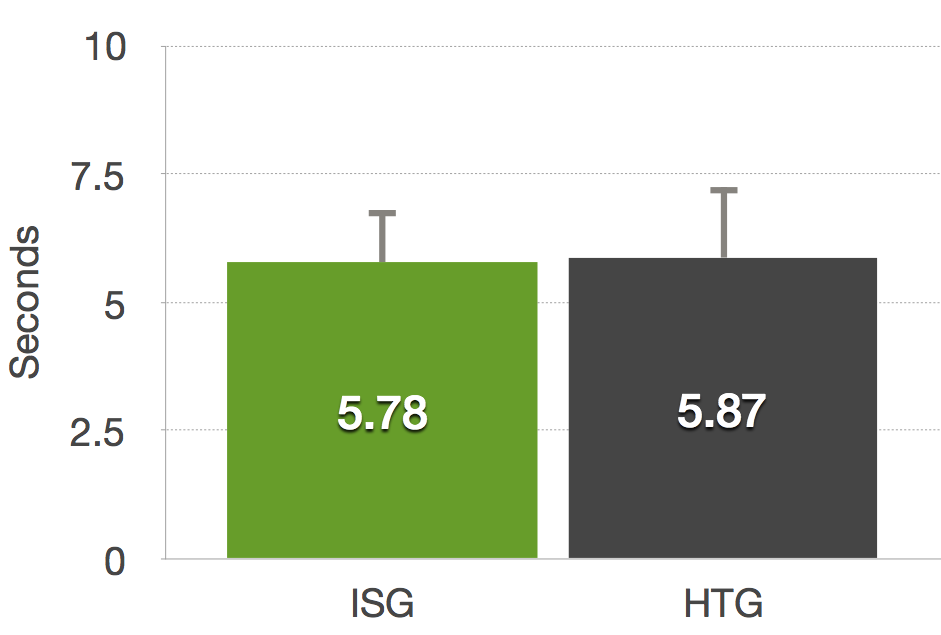
\includegraphics[width=1\linewidth]{Pictures/6_4_DIA_StandLeftGroupEffect}
		\subcaption{Stand Left Results}
		\label{fig:6_4_standLeftGroupEffect}
	\end{minipage}
	\hfill
	\begin{minipage}[t]{0.40\linewidth}
		\centering
		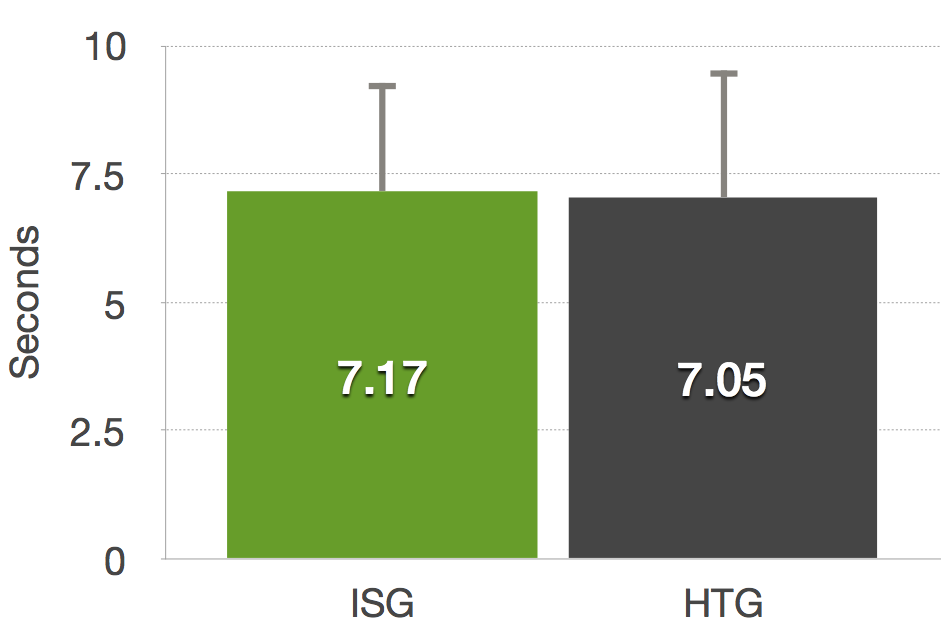
\includegraphics[width=1\linewidth]{Pictures/6_4_DIA_StandRightGroupEffect}
		\subcaption{Stand Right Results}
		\label{fig:6_4_standRightGroupEffect}
	\end{minipage}
	\hfill
	\begin{minipage}[t]{0.40\linewidth}
		\centering
		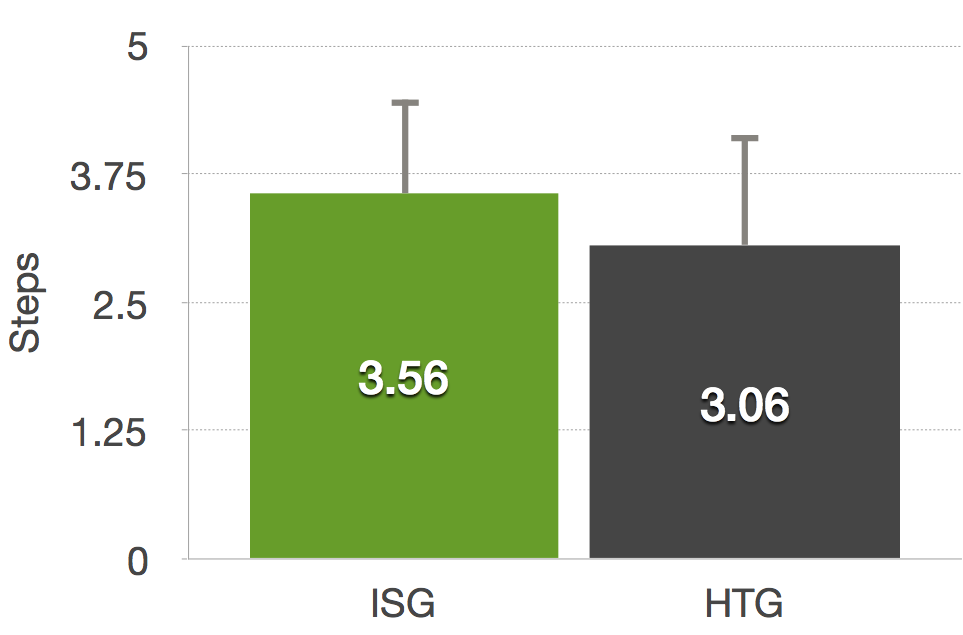
\includegraphics[width=1\linewidth]{Pictures/6_4_DIA_StepsLeftGroupEffect}
		\subcaption{Steps Left Results}
		\label{fig:6_4_stepsLeftGroupEffect}
	\end{minipage}
	\hfill
	\begin{minipage}[t]{0.40\linewidth}
		\centering
		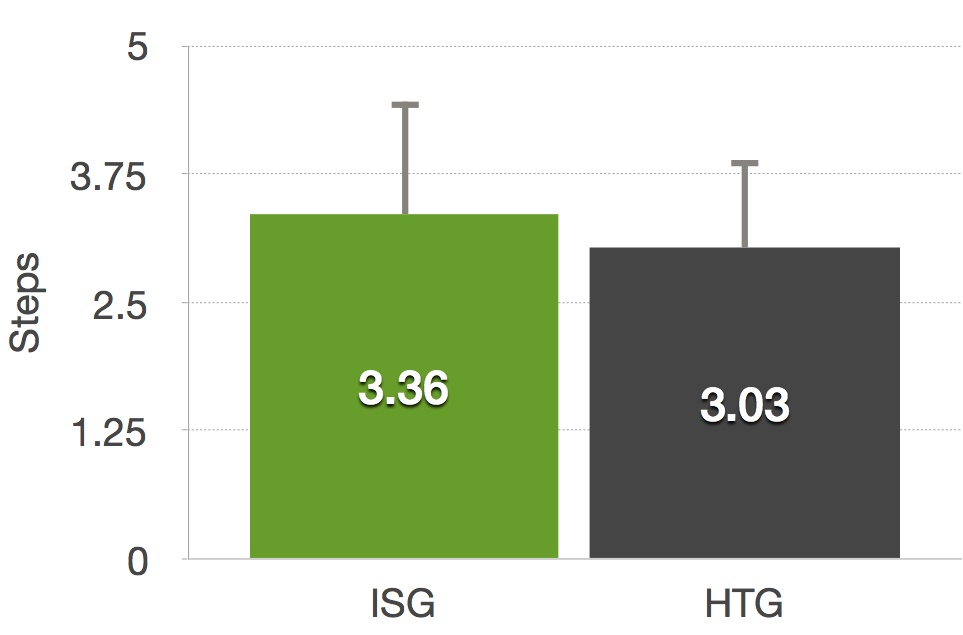
\includegraphics[width=1\linewidth]{Pictures/6_4_DIA_StepsRightGroupEffect}
		\subcaption{Steps Right Results}
		\label{fig:6_4_stepsRightGroupEffect}
	\end{minipage}
	\hfill
	\begin{minipage}[t]{0.40\linewidth}
		\centering
		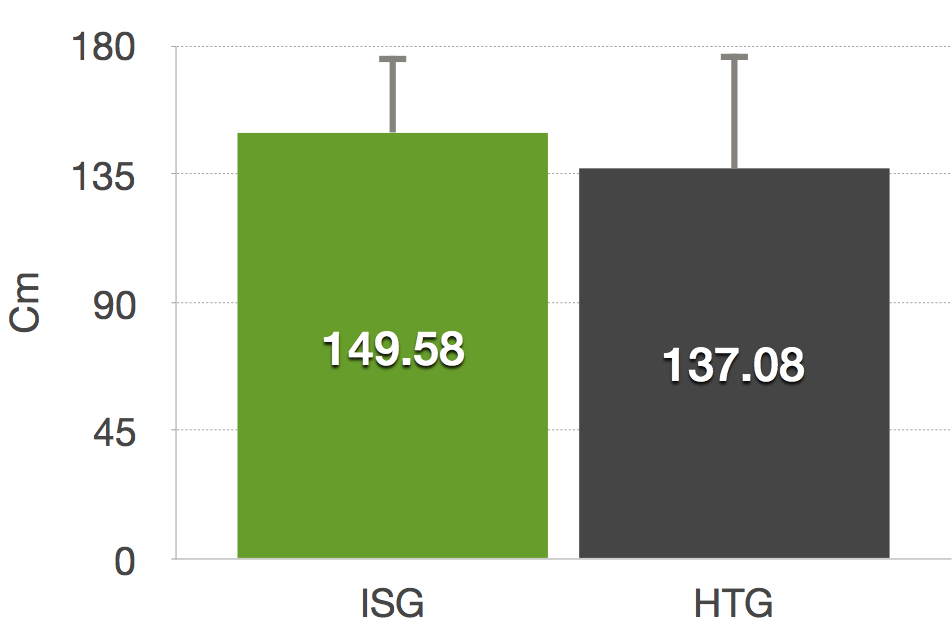
\includegraphics[width=1\linewidth]{Pictures/6_4_DIA_DistanceLeftGroupEffect}
		\subcaption{Distance Left Results}
		\label{fig:6_4_distanceLeftGroupEffect}
	\end{minipage}
	\hfill
	\begin{minipage}[t]{0.40\linewidth}
		\centering
		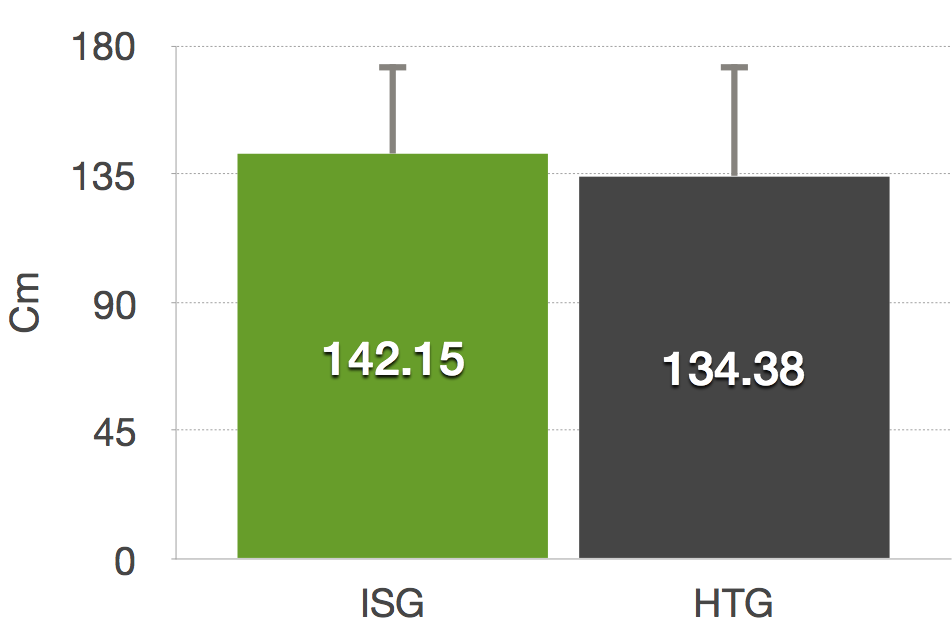
\includegraphics[width=1\linewidth]{Pictures/6_4_DIA_DistanceRightGroupEffect}
		\subcaption{Distance Right Results}
		\label{fig:6_4_distanceRightGroupEffect}
	\end{minipage}
	\caption{Scores for comparing the main effects of the group}
	\label{fig:6_4_mainEffectGroup}
\end{figure}

\subsubsection{Observations of the User Study}\label{6_4_slacklineObservations}
The observations during the study help to improve the system because each participant differs in their interaction with the system.
It is useful to consider these observations for further practice with the interactive slackline system and to improve it.

Since all participants had no real control of their body balance, it proves they were all beginners and had no further experience with the slackline.
Within the training participants were strengthened in their balance, learned to feel how their body behaves on the slackline, and how to counterbalance the body movement.
The post measurement proves the positive effect of this training since all participant improved in standing and walking more controlled on the line.

The virtual environment design gave a sense of a more playful training system with which participants enjoyed to interact with and motivated them.
Although there existed problems with the recognition of the Kinect, each participant had fun during the training and was motivated to accomplish each exercise.

The check list and timer in the exercise execution screen were mentioned as very helpful feedback indicators.
They provide support by notifying participants about the current status of their execution with clear audiovisual feedback.
It helped them to ensure their body was in the correct position for the exercise and when they are executing the exercise correctly.
This motivated participants because they were provided with immediate feedback about which part of the exercise is executed wrong and whether an exercise repetition was counted as correct.

On the other side there existed several tracking problems.
The black clothes of one participants absorb the infrared light of the Kinect, therefore making the trackability more difficult.
It would be helpful to inform participants not to wear any black clothes when using the Kinect.

Beside this, there was a problem with tracking participants while sitting on the slackline.
The leg was not properly tracked or mistaken with the slackline itself by the Kinect.
Furthermore, it was a very uncomfortable exercise for all participants.
Because of the way of how the problem exist, this exercise should be eliminated from the exercise list or replaced with exercises to train the first contact with the slackline in a more practicable way.

Going up and walking on the line resulted also in tracking problem.
The Kinect did not properly tracked the second step of the participants, which resulted in failures of the correct exercise execution.
This problem could be fixed by tracking the gestures with more persons that execute different variations of a correct exercise execution.

Concerning the interaction problems with scrolling in the exercise menu, it would be helpful to add an instruction on how to scroll a list in the system.

\subsubsection{Rating of Exercise Difficulty}
The ratings of the first level of the exercises matches the idea of slowly strengthen the general balance skill of the participants and preparing them for standing on a slackline.

However, the first two exercises of the second level were rated as very difficult.
This corresponds with the observations in the prior subsection \textit{\nameref{6_4_slacklineObservations}}, since in exercise 2.1 and 2.2 participant had to sit on the line.
They claimed these exercise were very uncomfortable or too difficult for them.

Exercise 3.1 is the same as 2.3 and exercise 3.2 is the same as 2.4, in which the participant learned to go up on the line.
Exercise 3.1 and 3.2 increased just in the time to hold the exercise.
Some participants noted they felt more secure to stand longer on the slackline after doing the short-time exercises.
Therefore they rated them similar to the prior exercise.

Further, the ratings follow a linear ongoing trend and match the intended exercise difficulty.
Overall this verifies the appropriate integration of the implemented exercises as an training model for beginners on a slackline.

\subsubsection{Semi-Structured Interview}
In general the participants noted the exercises were well structured such that they felt a learning progress.
The enjoyable environment gives a playful character for the training situation and the challenging exercises motivate them to reach their goal of accomplishing the exercise.
All participants had fun playing with the interactive slackline learning system and noted they would try it again.
They also recommend it for people who want to try slacklining.
Especially, because it is more structured as a gamified training system.

The application scenarios stated by the participants, like the usage in rehabilitation or as home trainer, verifies the system can be used to help and support persons, who have problems with their balance or want to improve it.